%----------------------------------------------------------------------------------------
%	SECTION 1.1
%----------------------------------------------------------------------------------------

\section{Path Connectedness.}

\begin{definition}
    A \textbf{path} in a topological space $X$ is a continuous map  $f:[0,1]
    \xrightarrow{} X$ such that $f(0)=a$ and $f(1)=b$ for some $a,b \in X$. We
    call  $a$ and  $b$ the  \textbf{endpoints} of $f$, we say $f$ goes
    \textbf{from} $a$  \textbf{to} $b$.
\end{definition}

\begin{definition}
    We call a topological space $X$ \textbf{path connected} if there exists a
    path from $a$ to $b$ for all $a,b \in X$.
\end{definition}

\begin{example}\label{2.8}
    The sphere $S^n$ is path connected.
\end{example}

\begin{lemma}\label{2.4.1}
    If $f:X \xrightarrow{} Y$ is a continuous map and $X$ is a path connected
    space, then  $f(X)$ is also path connected.
\end{lemma}

\begin{theorem}\label{2.4.2}
    If $X$ is a path connected space, then  $X$ is a connected space.
\end{theorem}
\begin{proof}
    Suppose that $X$ is disconnected. Then there exists a seperation of $X$ into
    disjoint open sets  $U$ and $V$. That is  $X=U \cup V$. Suppose however that
     $X$ is path connected. Then for points  $a \in U$ and  $b \in V$, there is
     a path  $f:[0,1] \xrightarrow{} X$ from $a$ to  $b$. Since  $[0,1]$ is a
     connected space, so is $f([0,1])$; however notice that $f([0,1])=(U \cap
     f([0,1])) \cup (f([0,1]) \cap v)$, which is a seperation of $f([0,1])$,
     since $U$ and  $V$ form a seperation.
\end{proof}

\begin{example}\label{2.9}
    The converse of theorem \ref{2.4.1} is not true in general. Consider the
    following two examples:
    \begin{enumerate}
        \item[(1)] Consider the subspace $X=(0 \times [0,1]) \cup G$ where $G$
            is the graph of  $\sin{\frac{1}{x}}$ on the interval $(0,2\pi]$. We
            have that $X$ is connected, since the component containing $G$ is
            closed, and $0 \times [0,1] \subseteq \cl{G}$. However, $X$ is not
            path connected. We call the space $X$ the  \textbf{topologists sine
            curve}.

        \item[(2)] Another example of a connected space in $\R^2$ that is not
            path connected is the  \textbf{topologist's whirlpool}.
    \end{enumerate}
\end{example}

\begin{lemma}\label{2.4.3}
    Every contractible space is path connected.
\end{lemma}

\begin{lemma}\label{2.2.4}
    A topological space $X$ is path connected if, and only if any two
    constant maps  $X \xrightarrow{} X$ are homotopic.
\end{lemma}

\begin{lemma}\label{2.2.5}
    If $X$ is a contractible space and  $Y$ a path connected space, then any two
    continuous maps  $X \xrightarrow{} Y$ are homotopic.
\end{lemma}
\begin{corollary}
    The continuous maps are nullhomotopic.
\end{corollary}

\begin{lemma}\label{2.4.6}
    If $X$ and  $Y$ are path connnected spaces, then so is  $X \times Y$.
\end{lemma}

\begin{lemma}\label{2.4.7}
    If $f:X \xrightarrow{} Y$ is a continuous map and $X$ is a path connected
    space, then  $f(X)$ is also path connected.
\end{lemma}

\begin{theorem}\label{2.4.8}
    If $X$ is a topological space, then the relation  $\sim$ defined on  $X$ by
     $a \sim b$ if, and only if there is a path from $a$ to $b$, is an
     equivalence relation.
\end{theorem}
\begin{proof}
    Consider the constant path $c:[0,1] \xrightarrow{} X$ where $c(x)=a$ for all
    $x \in A$.  $c$ is continuous, and  $c(0)=c(1)=a$. So $a \sim a$.

    Now suppose that for  $a,b \in X$, that  $a \sim b$. Then there is a path
    $f:[0,1] \xrightarrow{} X$ with $f(0)=a$ and $f(1)=b$. Consider the map
    $g:[0,1] \xrightarrow{} X$ defined by $g(t)=f(1-t)$. $g$ is continuous by
    composition, and $g(0)=f(1)=b$ and $g(1)=f(0)=a$, which makes $b \sim a$.

    Lastly, suppose that  $a \sim b$ and  $b \sim c$ for some  $a,b,c \in X$.
    Then there exist paths  $f:[0,1] \xrightarrow{} X$ and $g:[0,1]
    \xrightarrow{} X$ with $f(0)=a$, $f(1)=b$, and $g(0)=b$, $g(1)=a$. Now,
    consider the map $h:[0,1] \xrightarrow{} X$ defined by:
    \begin{equation*}
       h(t)=\begin{cases}
                f(2t), \text{ if } 0 \leq t \leq \frac{1}{2}    \\
                g(2t-1), \text{ if } \frac{1}{2} \leq t \leq 1
            \end{cases}
    \end{equation*}
    Notce that $f(\frac{1}{2})=g(\frac{1}{2})=f(1)=g(0)=b$, so the domains of
    $f$ and  $g$ coincide. Therefore by the pasting lemma, $h$ is continuous.
    Now, observe that  $h(0)=f(0)=a$, and that $h(1)=g(1)=c$. This makes $a \sim
    c$.
\end{proof}

\begin{definition}
    We define the equivalence classes of $X$ under path connectedness to be
    called \textbf{path components} of $X$.
\end{definition}

\begin{definition}
    We denote the collection of all path components of a topological space $X$
    to be  $pi_0(X)$; that is $pi_0(X)=\faktor{X}{\sim}$ (not necesarily as a
    quotient space), Moreover, we define the map $pi_0(f):pi_0(X) \xrightarrow{}
    pi_0(Y)$ to be the map taking the path component $C$ to the unique path
    component of $Y$ containing $f(C)$.
\end{definition}

\begin{theorem}\label{2.4.9}
    $pi_0:\Top \xrightarrow{} \Set$ is a funtor.
\end{theorem}
\begin{proof}
    Consider $1_X:X \xrightarrow{} X$ the identity on $X$. Let
    $\pi_0(X)=\{X_\alpha\}$ where $X_\alpha$ is a path component of $X$. We have
    that $pi_0(1_X):\pi_0(X) \xrightarrow{} \pi_0(X)$ sends $X_\alpha
    \xrightarrow{} X_\beta$ where $X_\beta$ is the unique path component of  $X$
    containing  $1_X(X_\alpha)=X_\alpha$. However, since $X_\alpha$ and
    $X_\beta$ are equivalence classes, we have  $X_\alpha \subseteq X_\beta$ if
    and only if  $\alpha=\beta$, i.e.  $X_\alpha=X_\beta$. This makes
    $pi_0(1_X)=1_{\pi_0(X)}$.

    Now let $f:X \xrightarrow{} Y$ and $g:Y \xrightarrow{} Z$ be continuous
    maps. Let $\pi_0(X)=\{X_\alpha\}$, $\pi_0(Y)=\{Y_\beta\}$, $\pi_0(Z)=
    \{Z_\gamma\}$ the collection of path components of $X$,  $Y$, and  $Z$,
    respectively. Now consider  $X_\alpha$ and  $Z_\gamma$ such that  $\pi_0(g
    \circ f)(X_\alpha)=Z_\gamma$. Then $Z_\gamma$ is the unique path component
    of  $Z$ containing  $g(f(X_\alpha))$. Now, if $Y_\beta$ is the unique path
    component of $Y$ containing $X_\alpha$, then $\pi_0(f)(X_\alpha)=Y_\beta$
    and we see that  $g(f(X_\alpha)) \subseteq g(Y_\beta)$. Moreover, if
    $Z_{\gamm'}$ is the unique path component of $Z$ containing  $g(Y_\beta)$,
    then $\pi_0(g)(Y_\beta)=Z_{\gamma'}$, and $g(Y_\beta) \subseteq
    Z_{\gamma'}$. But $g(f(X_\alpha)) \subseteq g(Y_\beta) \subseteq
    Z_{\gamma'}$; by above, and since path components partition their spaces,
    this makes $\gamma=\gamma'$. Thus  $Z_\gamma=Z_{\gamma'}$ and we have that
    $g(f(X_\alpha)) \subseteq g(Y_\beta) \subseteq Z_\gamma$. Therefore $Z_\gamma$
    is the unique path component of $Z$ containing both  $g(f(X_\alpha))$ and
    $g(Y_\gamma)$; that is $\pi_0(g)(Y_\beta)=Z_\gamma$, where
    $\pi_0(f)(X_\alpha)=Y_\beta$. This implies that $pi_0(g \circ f)=\pi_0(g)
    \circ \pi_0(f)$, which makes $\pi_0$ a functor.
\end{proof}
\begin{corollary}
    If $f \simeq g$, then  $\pi_0(f)=\pi_0(g)$.
\end{corollary}
\begin{proof}
    Suppose that $F:f \simeq g$ is a homotopy between the maps  $f:X
    \xrightarrow{} Y$ and $g:X \xrightarrow{} Y$. Let $C$ be a path component of
     $X$, then $C \times I$ is path connected by lemma \ref{2.4.6}. Thus by lema
     \ref{2.4.1}, $F(C \times I)$ is also path connected. Notice then that:
     \begin{equation*}
         f(C)=F(C \times 0) \subseteq F(C \times I)
     \end{equation*}
     and
     \begin{equation*}
         g(C)=F(C \times 1) \subseteq F(C \times I)
     \end{equation*}
     So the unique path connected component of $Y$ containing $F(C \times I)$
     contains both  $f(C)$ and $g(C)$. Therefore $\pi_0(f)=\pi_0(g)$.
\end{proof}
\begin{corollary}
    If $X$ and  $Y$ are topological spaces with the same homotopy type, then
    they have the same number of path components.
\end{corollary}
\begin{proof}
    Suppose that $f:X \xrightarrow{} Y$ and $g:Y \xrightarrow{} X$ are
    continuous maps with $g \circ f=1_X$ and  $f \circ g=1_Y$. Since $f$ is a
    homotopy equivalence, then  $[f]$ is an equivalence in $\hTop$. Restricting
     $\pi_0$ to $\hTop$, this also gives use that $\pi_0([f])$ is an equivalence
     in $\Set$. That is  $f$ is 1--1 and onto.
\end{proof}

\begin{definition}
    A topological space $X$ is  \textbf{locally path connected} if, for each $x
    \in X$, and every open neighborhood $U$ of  $x$ there is an open set $V$
    with  $x \in V \subseteq U$ such that any two points in  $V$ can be joined
    by a path in $U$.
\end{definition}

\begin{example}\label{2.10}
    Form the subspace $X$ of $\R^2$ by asjoining a curve from  $(0,1)$ to
    $(\frac{1}{2\pi}, 0)$ on the topologist's sine curve. Then  $X$ is path
    connected, but not locally path connected.
\end{example}

\begin{theorem}\label{2.4.10}
    A topological space is locally path connected if, and only if path
    components of open sets are open.
\end{theorem}
\begin{proof}
    Suppose that $X$ is locally path connectd, and lwet  $U$ be open in $X$. Let
     $x \in C$, where  $C$ s a path component of  $U$. Then there is an open
     $V$ with  $x \in V \subseteq U$ such that very point of  $V$ can be joined
     to  $x$ by a path in $U$. Thus each point of $V$ lies in the path component
     of $x$, which is $C$. Thus $V \subseteq C$, which makes  $C$ open.

     Conversely, suppose that path components of open sets in  $X$ are open. Let
      $U$ be an open set of  $X$, and for some  $x \in U$, let  $C$ be the path
      component of $x$ in $U$. Then we have $x \in C \subseteq U$. Since $C$ is
      open, this makes $X$ locally path connected.
\end{proof}
\begin{corollary}
    If $X$ is locally path connected, then its path components are open.
\end{corollary}
\begin{corollary}
    $X$ is locally path connected if, and only if for every $x \in X$, and each
    open neighborhood  $U$ of  $x$, there is an open path connected set  $V$
    with  $x \in V \subseteq U$.
\end{corollary}
\begin{corollary}
    If $X$ is locally path connected, then the connected components of every
    open set coincide with its path components. In particular the connected
    components of $X$ coincide with the path components of  $X$.
\end{corollary}
\begin{corollary}
    If $X$ is connected, and locally path connected, then  $X$ is connected.
\end{corollary}

\begin{definition}
    Let $A$ be a subspace of a topological space  $X$, and let  $i:A
    \xrightarrow{} X$ be the inclusion. Then $A$ is a \textbf{deformation
    retract} of $X$ if there is a continuous map  $r:X \xrightarrow{} A$ such
    that $r$ is a retraction of $X$; i.e. $r \circ i=1_A$ and  $i \circ r=1_X$.
\end{definition}

\begin{lemma}\label{2.4.11}
    Every deformation retract is a retract.
\end{lemma}

\begin{theorem}\label{2.4.12}
    If $A$ is a deformation retract of a topological space  $X$, then  $X$ and
    $A$ have the same homotopy type.
\end{theorem}
\begin{corollary}
    $S^1$ is a deformation retract of  $\com{\C}{0}$.
\end{corollary}
\begin{proof}
    For every $z \in \com{\C}{0}$, we can write $z$ as  $z=\rho e^{i\theta}$,
    where $\rho>0$, and  $0 \leq \theta \leq 2\pi$. Now, define
    $F:(\com{\C}{0}) \times I \xrightarrow{} \com{\C}{0}$ by taking $(\rho
    e^{i\theta},t) \xrightarrow{} ((1-t)\rho+t)e^{i\theta}$. Notce that $F$ is
    never  $0$, and that $F$ is continuous, with $F(\rho e^{i\theta},0)=\rho
    e^{i\theta}$, $F(e^{i\theta},1)=e^{i\theta}$. Moreover $F(\rho
    e^{i\theta},1)=F(e^{i\theta})=e^{i\theta}$. Writing $S^1$ as
    $S^1=\{e^{i\theta} : 0 \leq \theta \leq 2\pi\}$. We see that $F$ makes $S^1$
    into a deformation retract of $\com{\C}{0}$.
\end{proof}
\begin{corollary}
    $S^1$ has the same homotopy type as  $\com{\C}{0}$.
\end{corollary}

\begin{definition}
    Let $f:X \xrightarrow{} Y$ be a continuous map from a topological space $X$
    to a topological space  $Y$. Define
    \begin{equation*}
        M_f=\faktor{(X \times I) \cup Y}{\sim}
    \end{equation*}
    Where $(X \times I) \cup Y$ is a disjoint union, and $\sim$ is an
    equivalence relation defined by $(x,t) \sim y$ if $y=f(x)$ and  $t=1$.
    Denote the equivalece classes of $(x,t)$ by $[x,t]$. We call the quotient
    spce $M_f$ the  \textbf{mapping cylinder} of $f$.
\end{definition}

\begin{figure}[h]
    \centering
    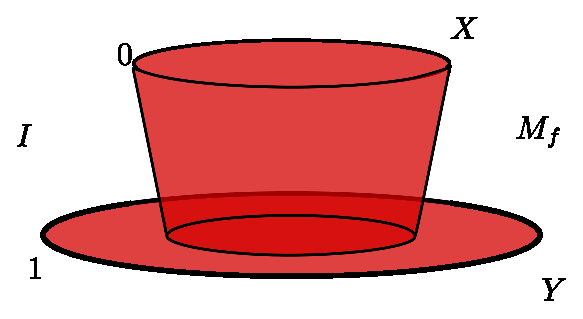
\includegraphics[scale=0.5]{Figures/Chapter2/mapping_cylinder.eps}
    \caption{The mapping cylinder of a continuous map $f:X \xrightarrow{} Y$.}
    \label{fig_2.2}
\end{figure}
